\documentclass{article} % For LaTeX2e
\usepackage{nips_adapted,times}
\usepackage{hyperref}
\usepackage{url}
\usepackage{graphicx}

\title{Text generation and Style Transfer\\Data Vaders - Group 17}


\author{
Soumye Singhal \\
150728 \\
\texttt{soumye@iitk.ac.in}\\
\And
K. Siddarth \\
150312 \\
\texttt{siddarth@iitk.ac.in}\\
\And
Prakhar Agarwal \\
150499 \\
\texttt{pkhrag@iitk.ac.in}\\
\AND
Abhibhav Garg \\
150010 \\
\texttt{abhibhav@iitk.ac.in}\\
\And
Nishit Asnani \\
Mentor
}

\newcommand{\fix}{\marginpar{FIX}}
\newcommand{\new}{\marginpar{NEW}}

\nipsfinalcopy

\begin{document}

\maketitle

\section{Introduction and Motivation}
Our project has two parts.\\
The first part deals with \textbf{Text Generation}. Text generation is the fundamental task in Natural Language Processing which aims to produce a natural language text in order to meet specified communicative goals. It takes the non-linguistic representation of information as input and outputs text, documents, stories etc. It has a diverse set of applications ranging from image captioning to text summarization. We aim to
use current state of the art Deep Learning techniques to capture the artistic style of an author and
then generate text in that same style.  Formally, given a starting sentence and a target author (say
JK Rowling or Shakespeare), we use text generation methods to complete a paragraph in the style of
that author. We compare the performance of RNN's and LSTM's. We also see how the performance changes with the change in the architecture.\\
The second part deals with \textbf{Style Transfer}. We want to use deep learning based seq2seq models to change the style of a given content from that of the original author to that of a new target author. More formally, given some text of any author, we want to convert it to the style of another, while still preserving the meaning of the text. We experiment with our original idea and analyze its performance.\\
We think that pursuing this task will bring us closer to an algorithmic understanding of how our brains are able to create and perceive artistic literature and how it captures style.
% Our project is on Text Generation and Neural Style Transfer. Given a story in the style of one author, we designed a model which takes the text in the style of one author and convert it to that of another author. We experimented with different models to find the best one. Our model 





% \subsection{Subsection (if any) Name}


\section{Related/Previous Work}
% A lot of work has been done on text generation. Our work is mostly inspired by A. Karpathy \cite{karpathy}. He trained a character-level language RNN model using multi-layer LSTMs. RNNs contain cycle in their network. At every time-stamp, a character is fed into it and it predicts the next character.
Our work on text generation was inspired by Karpathy's\cite{karpathy} work on text generation using character level models. In his article, he goes over the effectiveness of recurrent models in text generation.

% Any recurrent neural network basically works by taking in an input $in$ at a time-step $t$, and a hidden state function from the previous time-step, with which it predicts the next output. \\

Our work on style transfer of text was inspired by Gatys et. al.'s\cite{DBLP:journals/corr/GatysEB15a} work on style transfer of painters in vision.\\
There has not been much work on transferring the style of the text of one author to another. Hu et. al.\cite{DBLP:journals/corr/HuYLSX17} did controlled text generation using Variational Autoencoders\cite{2013arXiv1312.6114K}. But their work dealt with generating any paraphrase of a given input. What we want to do is create a specific type of paraphrase, not just any paraphrase. In that respect, this problem is similar to machine translation, where we want to translate text from a given input language to a different output language. Sequence to sequence encoder-decoder models have proven to be very successful in that regard. Bahdanau et. al. \cite{DBLP:journals/corr/BahdanauCB14} gave state-of-the-art results in machine translation in 2014. % TODO: check 
% Our model for style transfer is an encoder-decoder model augmented with attention.
\newpage

\section{Models}

\subsection{Text generation}
Our text generation model is based on simple Recurrent Neural Network(RNN) based language model trained on the text of the target author. The RNN learns to predict the next word given the previous context. Since it's trained on the target authors corpus, when we feed in the context of our input string it starts to predict the next word in the style of that author. We then keep on picking this predicted word to generate and complete the text in the style of that author.\\
\begin{figure}[ht!]
    \centering
    \includegraphics[width=0.8\linewidth]{1.pdf}
    \caption{Recurrent Neural Network- At each timestamp, a character and some computation of last time-stamp is given as input to compute the next character.}
\end{figure}
In the model described in this Figure, $h_i$ denote hidden state of the RNN. The network outputs a distribution over vocabulary, from which we sample out the output tokens $out_i$.
\begin{itemize}
        \item $w_i$ - input tokens of source text    
        \item $h_i$ - Encoder hidden states
        \item $P_{vocab} = softmax(Vh_i + b)$ is the distribution over vocabulary from which we sample $out_i$
        \label{fig:lstm}
\end{itemize}
The recurring unit can be either a vanilla RNN or an LSTM unit. LSTM's(Long Short Term Memory networks) improve on RNN's by maintaining a gating system, which mitigates the vanishing and exploding gradient problem experienced by vanilla RNNs.
  \begin{figure}[h]
%   \caption{A Basic LSTM Unit with it layers. }
  \centering
  \includegraphics[width=0.8\linewidth]{5.pdf}
  \end{figure}
  \footnote{Image taken from \texttt{colah.github.io}}
% \newpage
%     \textbf{Input Gate Layer} 
%     \begin{itemize}
%         \item $i_t = \sigma(W_t[h_{t-1},x_t] + b_i)$
%         \item $\widetilde{C_t} = tanh(W_i[h_{t-1},x_t] + b_c)$
%         \item $C_t = \widetilde{C_t} \otimes t_t + C_t$
%     \end{itemize}
%         \textbf{Forget Gate Layer}
%     \begin{itemize}
%         \item $f_t = \sigma(W_f[h_{t-1},x_t] + b_f)$
%         \item $C_t = C_t \otimes f_t$
%     \end{itemize}
%     \textbf{Output Gate Layer}
%     \begin{itemize}
%         \item $o_t = \sigma(W_o[h_{t-1},x_t] + b_o)$
%         \item $h_t = o_t * tanh(C_t)$
%     \end{itemize}
We can implement this RNN network in two ways. The inputs can be either characters or words. We correspondingly get either a character RNN or a word RNN. We experimented with both of them and compared their performance.
We also experimented with different recurrent units like RNN's and LSTM's, varying stacked layers and varying hidden layer size. We present a comparison of results in the experiments section. We saw that our model performs best for word LSTM, with 512 size hidden layer and 3 stacked layers.

\subsection{Style Transfer}
Our model for style transfer from one author to another is based on the basic sequence to sequence encoder-decoder model with attention. These models are used to map an input sequence of words to another target sequence of words of possibly different vocabulary. They are used in tasks like machine translation, paraphrasing and text summarization.\\
Sequence to sequence models consist of an encoder and a decoder. The input is passed through the encoder to get a latent representation(called a thought vector). This is then passed through a decoder which decodes the latent representation to give the output.

\begin{figure}[th!]
    \includegraphics[width=1.0\columnwidth]{seq2seq2.png}
    \caption{A seq2seq model}
\end{figure}

\textbf{Attention Mechanism}\\
  The basic encoder-decoder model performs moderately well on very short sequences but it fails to scale up. 
    \begin{itemize}
      \item  The main bottleneck is the fixed sized encoding of the input string, which is the LSTM output of the last time-step. Due to it's fixed size it is not able to capture all the relevant information of the input sequence as the model sizes up. 
      \item At each generation step, only a part of the input is relevant. So how does the model decide which part of the input encoding to focus on at each generation step?
      \item At each step, the decoder outputs hidden state $h_i$, from which we generate the output.
    \end{itemize}
 
  The solution to this problem is using the attention model\footnote{Image stylized from https://talbaumel.github.io/attention/}. This model calculates the importance of each input encoding for the current step by doing a similarity check between decoder output at this step and input encodings. Doing this for all of the input encodings and normalizing, we get an importance Vector. We then convert it to probabilities by passing through softmax. Then we form a context vector by multiplying with the encodings.
  \begin{itemize}
      
      \item $importance_{it} = V* tanh(e_iW_1+h_tW_2+b_{attn})$.
      \item Attention Distribution $a^t = softmax(importance_{it})$
      \item  ContextVector $ h^{*}_t = \sum_i e_i*a^t_i$
      
  \end{itemize}
  \begin{figure}[!h]
  % \caption{The Baseline Attention model used by bahdanau et al.}
  \centering
  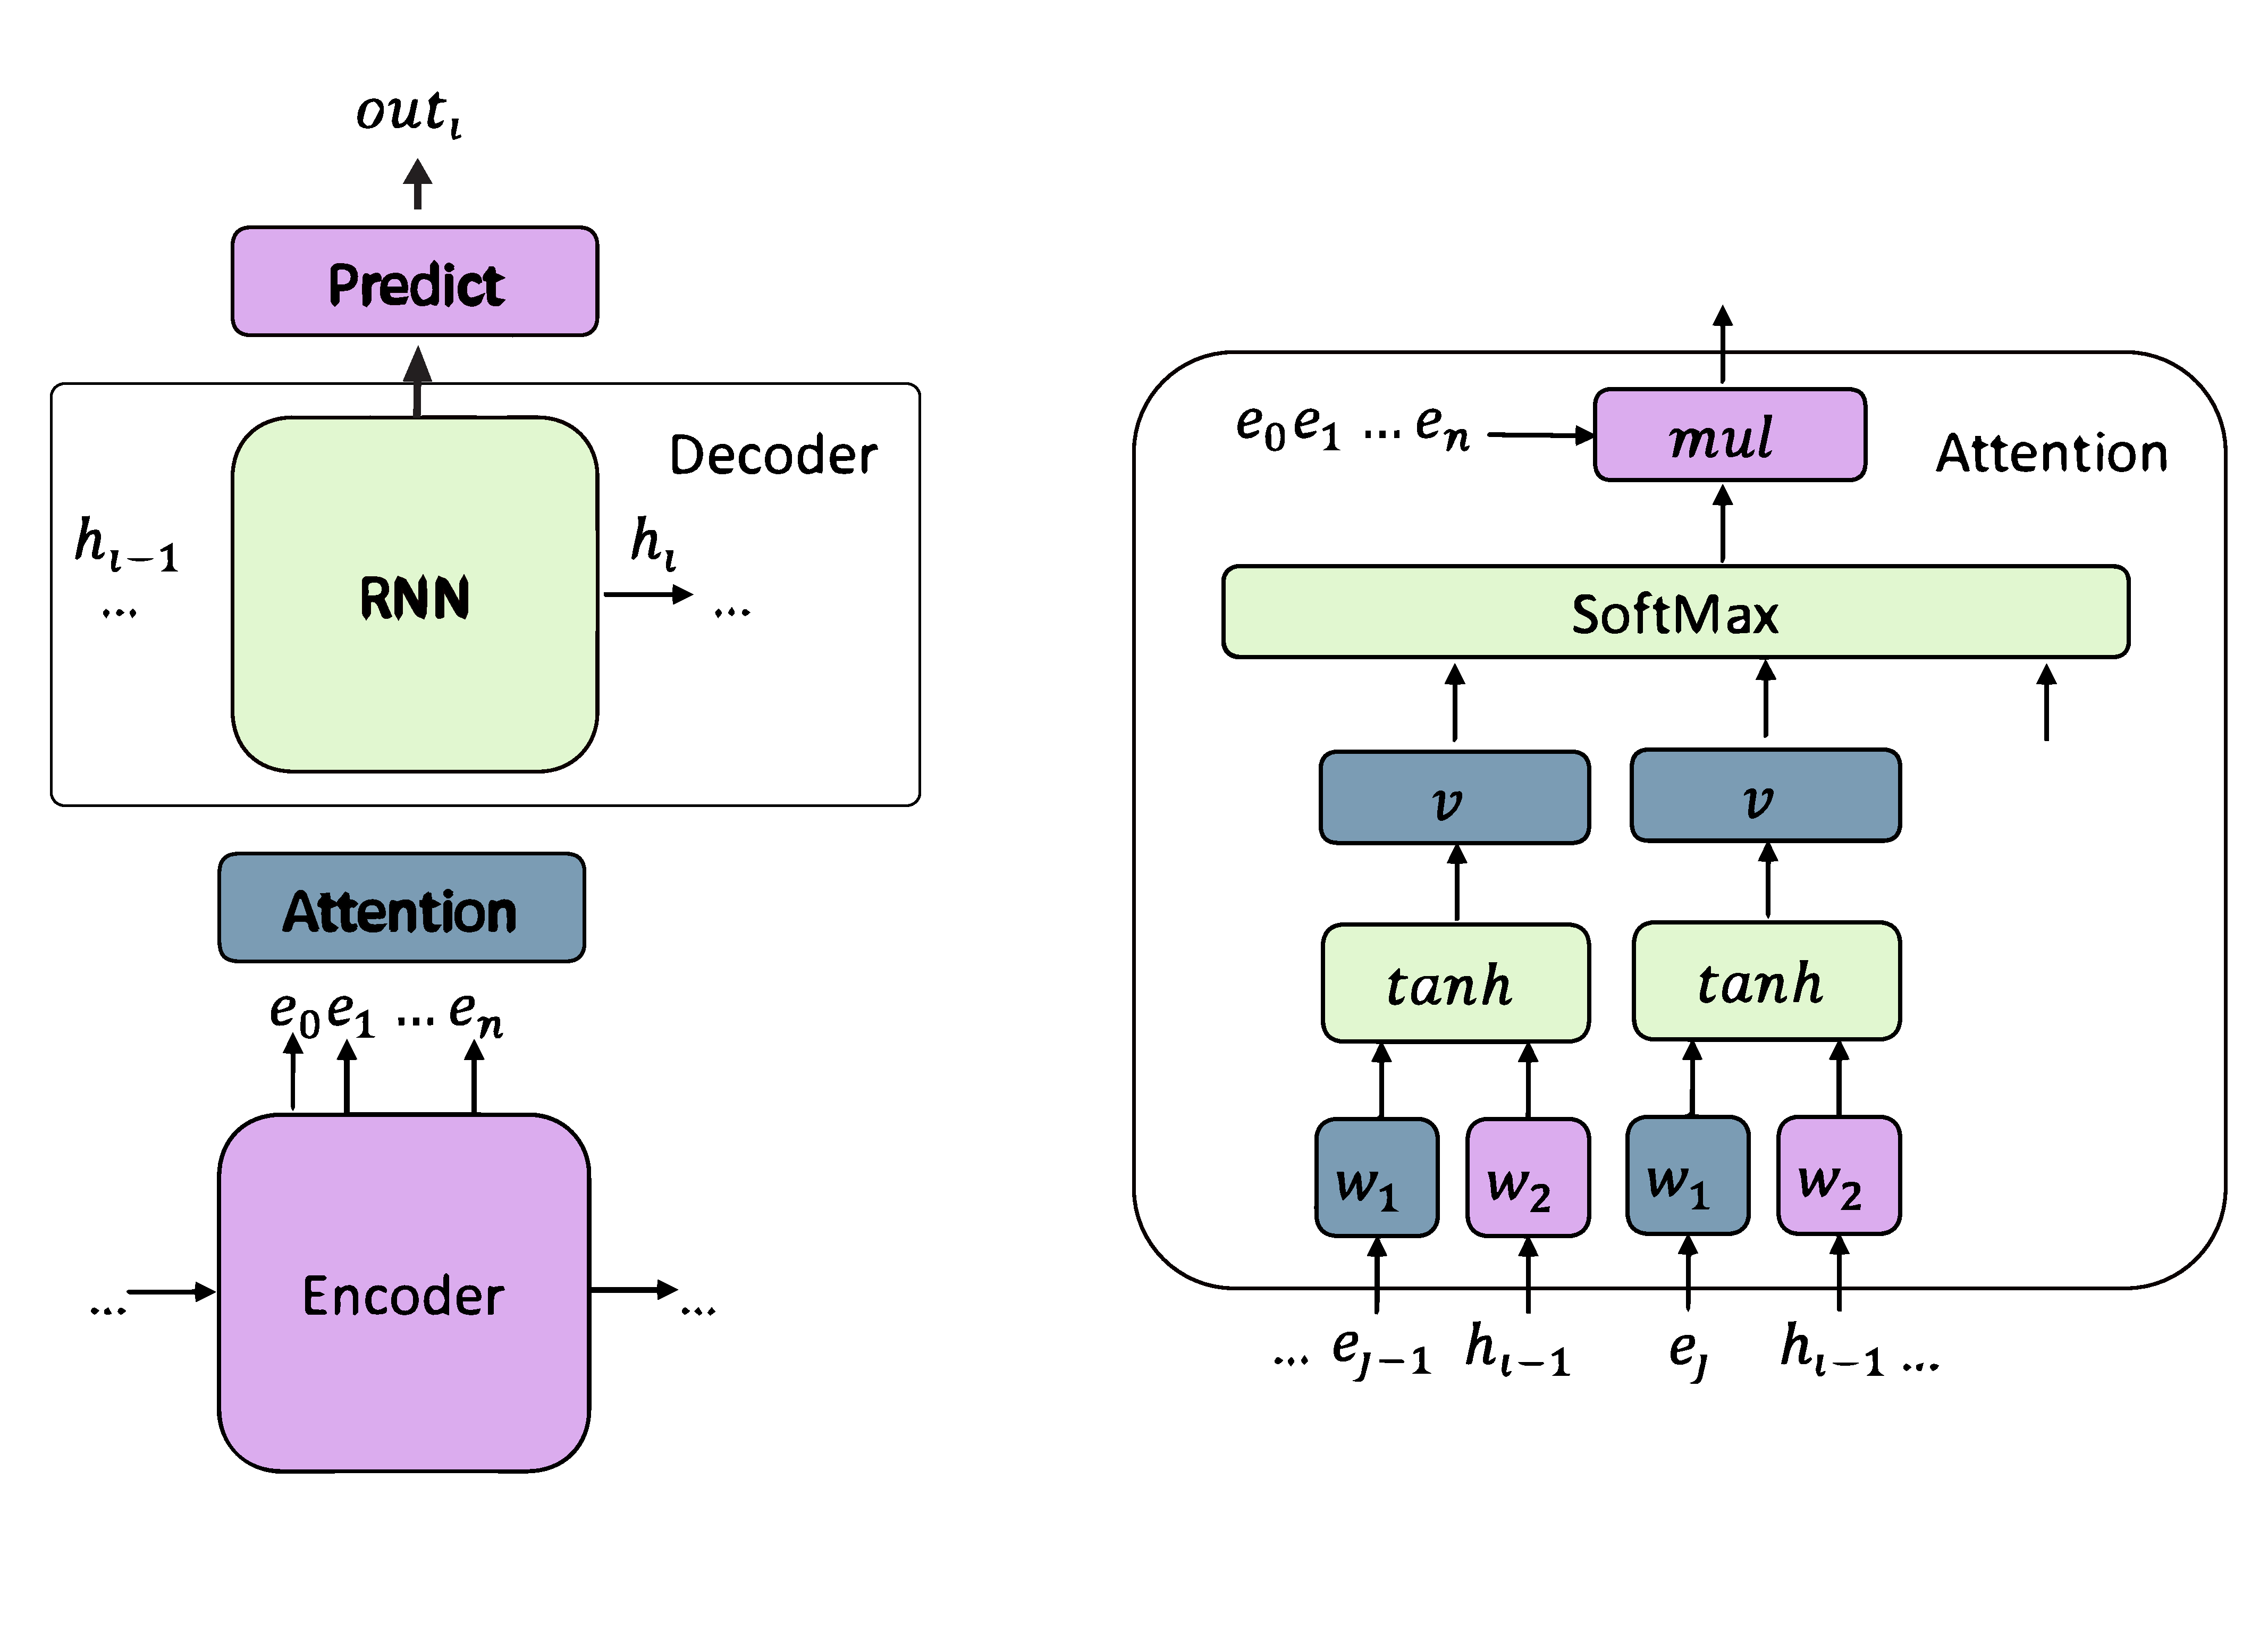
\includegraphics[width=0.8\linewidth]{7.pdf}\\
  \end{figure}
Context Vector is then fed into two layers to generate distribution over the vocabulary from which we sample.
  \begin{itemize}
    \item $P_{vocab}(w) = softmax(V'(V[h_t,h_t^*] + b) + b')$
    \item For the loss at time step $t$, $loss_t = -\log P(w_t^*)$, where $w_t^*$ is the target word.
    \item $LOSS = \frac{1}{T} \sum_{t=0}^{T} loss_t$ is the total loss across all time-steps.
    \item We then use the Back-propagation through time Algorithm to get the gradients and then apply any of the popular Gradient Descent algorithms to minimize the loss and learn good parameters.
\end{itemize}
% \textbf{Step 1}
% \begin{itemize}
%     \item We make a seq2seq encoder-decoder work as an auto-encoder first. That is given an input sentence, we train it output the same sentence.
%     \item We train this for \textbf{Author 1}. We did this for \texttt{Agatha Christie} and \texttt{Shakespeare}
%     \item As these models can't handle multiple sentences well, we only train these on single sentence to single sentence
% \end{itemize}
 
% \textbf{Step 2}
% \begin{itemize}
%     \item Once the seq2seq auto-encoder is trained, we input the sentence of \textbf{Author 2} , in our case \texttt{Sir Arthur Conan Doyle}.
% \end{itemize}
\subsection*{Our Idea}
We make a seq2seq encoder-decoder work as an auto-encoder first. That is given an input sentence, we train it to output the same sentence. We did this for \texttt{Agatha Christie}, \texttt{Shakespeare} and \texttt{Arthur Conan Doyle}. As these models can't handle multiple sentences well, we only train these on single sentence to single sentence. Once the seq2seq auto-encoder is trained, we take the input from Author 1(say \texttt{Arthur Conan Doyle}), and encode it using the encoder trained on Author 1. We then take the thought vector generated by it and pass it through the decoder trained on Author 2(say \texttt{Agatha Christie}).\\


\subsection*{Why we think it should it work?}
An autoencoder seq2seq network would first learn a good encoding of the sentence and then using that it learns to regenerate the sentence. Therefore, while training on an author the network needs to encode the sequence in general way such that it's possible to recreate the sequence from that encoding. The decoder which is working with the encoder also has to learn to decode that sequence and learns the structure of the sentence that doesn't vary from sentence to sentence. Therefore,
it makes sense for the model to encode only the content part of the sentence since the style remains constant for a given author(so the encoder would prefer to encode the more informative part, i.e. the content). And then the decoder can learn to recreate the given encoded content in the style of that particular author. So if we have two auto-encoder seq2seq models trained on two different authors, we can club the encoder of one and the decoder of another to get a model that does style transfer from one author to another

In our \textbf{final model}, we used a bi-directional LSTM for encoder and simple LSTM for decoder. We used hidden state size of 1024 and 2 stacked layers of LSTMs. The embedding size for the words was 500. We used beam search with a beam width of 5 to sample, and the maximum decode length was 300.

% \textbf{Why should it dwork?}
% \begin{itemize}
%     \item eWe think that while training on the first author, the network would first learn a good encoding of that sentence. And then using that encoding it needs to learn regenerate the sentence.
%     \item So it makes sense for the model to encode only the content part of the sentence in the encoding because style is same for the author and that can be learned by the decoder.
%     \item We use different weights for encoder and decoder.
%     \item So when, we feed in the sentence of second author it's content gets encoded by the encoder.
%     \item Then the decoder styles that content in the style of the first author
% \end{itemize}

% \textbf{Parameters}
% \begin{itemize}
% \item Bidirectional LSTM
% \item Size = 1024
% \item Depth = 2
% \item Embedding size = 500
% \item beam width = 5
% \item max decode step = 300
% \end{itemize}
 
% \textbf{How good is our Auto-Encoder}
% \begin{itemize}
%     \item We use the \texttt{BLEU} metric to test how well our model does self encoding
%     \item We got a \texttt{BLEU} score of $55.13$, meaning it does the autoencoding pretty well
% \end{itemize}
 
\section{Dataset}
For the text generation part of our work, we used the TinyShakespeare dataset. It contains the concatenation of the works of \textbf{Shakespeare}. There are  40k sentences in the dataset.
\par
For the style transfer part, we took our data from Project Gutenberg.\cite{gutenberg} We collected the works of \textbf{Sir Arthur Conan Doyle} and \textbf{Agatha Christie} from Project Gutenberg to make a tiny dataset for each author, each of which had roughly 50k sentences.

\section{Tools and Libraries used}
We used Tensorflow to code our project. We used Google's NMT code \cite{luong17} as a boilerplate for seq2seq models. We coded the character/word RNNs ourselves from scratch.

\section{Experiments}

\subsection*{Hyperparameter Tuning}
We did hyperparameter tuning(depth and size of the model) manually. We tested it for a few cases to find the optimal value.


\subsection*{Character vs Word level RNN} 
First, we wanted to compare the effectiveness of character level language models versus word level models. 
We trained two recurrent neural net models, one on trained on characters and one on words. For both, we used 3-layer stacked LSTMs with 512 hidden nodes. These were the results we got:

\emph{Word Level}\\
\framebox{\parbox{\dimexpr\linewidth-2\fboxsep-2\fboxrule}{% 

King VI: First Citizen:  And will will tell you, I have not I is to be content; it are not that is a more than all the writing. \\ DUKE OF YORK: My lord, I am a bond, and we is the writing.\\ DUKE OF YORK: What is the writing.
}}
\\
\emph{Character Level}\\
\framebox{\parbox{\dimexpr\linewidth-2\fboxsep-2\fboxrule}{

\textbf{KINGequeses}, wifely
A mighty \textbf{vanagy} died, and is it \textbf{sotis} being note but by flatter, which,
I rather be! Hear over-blown swifled by
}
}

We can see that the character level model performs admirably; it is able to learn the syntactic structure of the text, and even some commonly used words like \emph{being}, \emph{which}, \emph{be}, etc. But it still conjures up new words, like \emph{vanagy}. This is not a problem with the word level model. 
\subsection*{Depth}
Next, we wanted to find the optimal depth for our model. Curiously, we found that on using a vanilla RNN stacked with 3 layers and 512 hidden nodes performed visibly worse than a 2 layer stacked RNN with the same hidden node width.

\emph{2 layer vanilla RNN}\\
\framebox{\parbox{\dimexpr\linewidth-2\fboxsep-2\fboxrule}{
KING RICHARD III: Ay, if you know the general is not so far with me. \\ QUEEN ELIZABETH: My lord, I will not not a man of such good Than not to see him in the Duke of York.\\ KING RICHARD III: Ay, but you will not be a traitor to the people, And yet thou art a soldier, and that is not so much with me for his eye.}}

\emph{3 layer vanilla RNN}\\
\framebox{\parbox{\dimexpr\linewidth-2\fboxsep-2\fboxrule}{
KING of of of of of of of of of of of of of of of of of of of of of of of of of of of of of of of of of of of of of of of of of of of of of of of of of of of of of of of of of of of of of of of of of of of of of of of of of of of of of of of of of of of of of of of of of of of of}}

This problem does not arise when we use LSTMs instead of RNNs

\emph{3 layer LSTM}\\
\framebox{\parbox{\dimexpr\linewidth-2\fboxsep-2\fboxrule}{
King VI: And will will tell you, I have not I is to be content; it are not that is a more than all the writing.\\ DUKE OF YORK: My lord, I am a bond, and we are the writing.\\ DUKE OF YORK: What is the writing}}

We believe the 3-layer LSTM outperforms the 3-layer RNN because gradients vanish much faster in vanilla RNN's than in LSTM's. During training of recurrent units, we want that the error to be back-propagated over all the time steps. With RNN's, the gradients very quickly tend to zero, meaning RNN's cannot learn long-term dependencies very well.\\ With the 2-layer RNN, the gradients have to be back-propagated over fewer layers compared to the 3-layer RNN, meaning fewer of the weights tend to zero. This allows the 2-layer RNN to perform better.

\subsection*{Style Transfer}

We trained two seq2seq models, one on \texttt{Conan Doyle} and one on \texttt{Agatha Christie}. We then passed the input text(Sherlock Holmes) through the encoder of \texttt{Conan Doyle} to get the thought vector. This was then given as input to the decoder of \texttt{Agatha Christie}\\

To measure how well our encoder-decoder model does auto-encoding, we calculated the \texttt{BLEU} score. It essentially measures n-gram overlap between two texts, so higher \texttt{BLEU} score will mean better auto-encoding quality. We got a score of \textbf{55.13}\%. This indicated that the encoder performs decently, but can be improved with more training data. \\
 

\subsection*{Results}
    \textbf{Sherlock Holmes (Original)}\\
    \framebox{\parbox{\dimexpr\linewidth-2\fboxsep-2\fboxrule}{
\textbf{Absolutely none.}
None. 
No sign of it? 
Come in !  said Holmes .
Seven !  I answered .
She will not sell . 
\textbf{And I.} 
My own seal . 
We have tried and failed . 
Stolen , then . 
I was mad - insane . 
To ruin me . 
We were both in the photograph . 
    }} 
    
    \textbf{Generated}\\
    \framebox{\parbox{\dimexpr\linewidth-2\fboxsep-2\fboxrule}{
    \textbf{Absolutely no}.
    None .
     No sign of it ? 
    Come in !  said . 
    Lord ! & I answered .
    She will not see . 
    \textbf{And me.}
    My mother. 
    We have come and rushed . 
    Welcome , then . 
    I was mad - . 
    To me me . 
    We both were in the photograph .
}}

\textbf{Sherlock Holmes (Original)}\\
\framebox{\parbox{\dimexpr\linewidth-2\fboxsep-2\fboxrule}{
What do you make of that ? asked Holmes .
 \textbf{I am about to be married} . 
 \textbf{I think that I had better go} , Holmes . 
 My private note-paper . 
 No legal papers or certificates ? 
 I promise ,  said Holmes .
I carefully examined the writing , and the paper upon which it was written .
}}
 

\textbf{Generated}\\
\framebox{\parbox{\dimexpr\linewidth-2\fboxsep-2\fboxrule}{
 What do you make of that ?  asked asked.
 \textbf{I am going to be married} .
 \textbf{I think that I had really go} , I had
 My private private.
 No girl or or two ? 
 I dare , said gruffly .
I carefully the man , and the paper paper which it was written .}}

As we can see, the conversions are not very good. There are some examples(the highlighted ones) where we can see that the structure of the sentence changes, but the meaning is (mostly) maintained. Also, we have no way of evaluating how good our translated texts are, given that there is not much text on the same content written by two different authors. \\
We also tried to convert Sherlock Holmes to Shakespeare(since the language used is so different, it would be much easier to see if the style was transferred), but due to their vocabularies being so different, we got junk.

 
\section{Future Work}
There is a lot of scope for extending the style transfer model. There are several shortcomings of this model that can be addressed. We noted that the model has struggle with the words that aren't present in the target author's vocabulary. So instead of outputting a garbage work there, we can use a pointer-generator network which learns to copy a word from the input sequence and give that as the predicted output instead. \par
Another drawback of our model is that the model has to learn the word embeddings layer itself based on the training data. But since in our case the data is scarce for the model to learn very good word representations, we can user pre trained word-vectors like word2vec of GloVe in our model instead.
\par
We can also use ideas from controlled generation of text to manually append a control variable to the encoding and then append a discriminator to the sequence so as to force the model to change the behavior of the output sequence based on the control variable we provide during testing. We can use this control variable to control various aspects of the style of an author.
% \subsubsection*{Referanences}
% % may use bixtex to automatically generate the list of references or
% % enter these manually below
% 
% \small{
% [1] Reference 1
% 
% [2] Reference 2
% }

\bibliography{772a_project}
\bibliographystyle{plain}

\end{document}
